\documentclass[12pt,a4paper]{article}
\usepackage[T1]{fontenc}
\usepackage[utf8]{inputenc}
\usepackage{amsmath,amssymb,amsfonts,amsthm,mathtools}
\usepackage{graphicx,float,geometry,hyperref,enumitem,xcolor}
\geometry{margin=2.5cm}

% ── Theorem environments ──
\theoremstyle{definition}
\newtheorem{definition}{Définition}[section]
\theoremstyle{remark}
\newtheorem{remarque}{Remarque}[section]

% ── Macros ──
\newcommand{\etat}{\mathit{état}}
\newcommand{\couleur}[1]{\mathit{couleur}_{#1}}

\title{\textbf{Cours 9 — Algorithmique distribuée et parallélisme}\\
       \large Détection de terminaison}
\date{18 mars 2026}
\author{}

\begin{document}
\maketitle
\tableofcontents
\bigskip

% ══════════════════════════════════════════════════════
\section{Détection de terminaison}
% ══════════════════════════════════════════════════════

Le système utilise des \textbf{messages de contrôle}. Il doit annoncer que
l'application est terminée si c'est le cas, c'est-à-dire si
\begin{itemize}
  \item tous les processus de l'application sont \emph{passifs}, et
  \item il n'y a pas de messages de travail en transit.
\end{itemize}

\paragraph{Problème.}
On a une application distribuée qui échange des messages (messages de travail).
\begin{itemize}
  \item Quand un processus reçoit un message de travail, il devient
        \emph{actif}.
  \item S'il ne reçoit pas d'autres messages de travail, un processus actif
        devient \emph{passif} dans le futur.
\end{itemize}

\begin{definition}[Sûreté]
  Le système n'annonce pas de fausse terminaison.
\end{definition}

\begin{definition}[Vivacité / Équité]
  Le système doit annoncer la terminaison au bout d'un nombre fini
  d'opérations.
\end{definition}

\paragraph{Hypothèse.}
Anneau orienté unidirectionnel, communications instantanées.

% ── Subsection ──
\subsection{Preuve par invariant}

On exhibe un \textbf{prédicat} $\mathcal{P}$ tel que :
\begin{enumerate}
  \item $\mathcal{P}$ est vrai dans la configuration initiale ;
  \item quand $\mathcal{P}$ est vrai dans une certaine configuration, cela
        implique que le problème est résolu.
\end{enumerate}

% ══════════════════════════════════════════════════════
\section{Algorithme de Dijkstra}
% ══════════════════════════════════════════════════════

\subsection{Règles}

Les processus $p_0, p_1, \ldots, p_{n-1}$ sont arrangés en anneau orienté
unidirectionnel.

\begin{figure}[H]
  \centering
  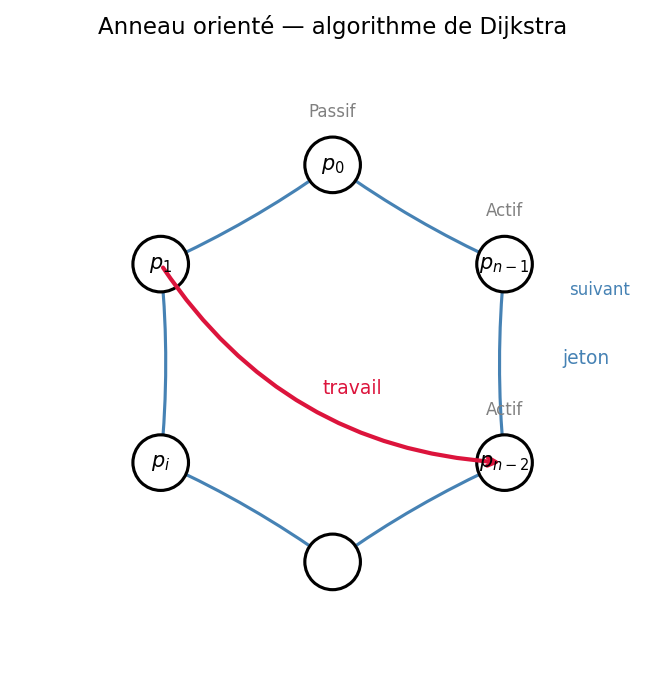
\includegraphics[width=0.58\textwidth]{figures/fig_ring_dijkstra.png}
  \caption{Anneau orienté unidirectionnel. Les flèches bleues indiquent la
           circulation du jeton (sens des indices décroissants). La flèche
           rouge représente un message de travail émis par un processus actif.}
  \label{fig:ring}
\end{figure}

\noindent Les règles sont les suivantes :
\begin{description}[leftmargin=2.5em]
  \item[$R_1$] Un processus a une couleur, \textbf{blanc} ou \textbf{noir},
               initialement blanc.
  \item[$R_2$] Le jeton a une couleur, blanc ou noir, initialement blanc.
  \item[$R_3$] Un processus qui reçoit un message de travail devient
               \textbf{noir}.
  \item[$R_4$] Seuls les processus \emph{passifs} transmettent le jeton.
  \item[$R_5$] Un processus \textbf{blanc} transmet le jeton (couleur du
               jeton inchangée). Un processus \textbf{noir} transmet le
               jeton \emph{noir}, et redevient blanc.
  \item[$R_6$] Si le jeton revient blanc à $p_0$, lui-même blanc et passif,
               $p_0$ \textbf{annonce la terminaison}.
\end{description}

\subsection{Pseudo-code}

\paragraph{Application.}
\begin{itemize}
  \item Lors d'un envoi d'un message de travail par $p$ reçu par $q$ :
        $\etat := \mathit{actif}$ \quad (transmission instantanée).
  \item Spontanément : $\etat := \mathit{passif}$.
\end{itemize}

\paragraph{Lors de l'envoi d'un message de travail par $p$ reçu par $q$ :}
\begin{align*}
  \couleur{p} &:= \mathit{noir} \\
  \etat_q     &:= \mathit{actif}
\end{align*}
\[
  \text{Quand } \etat = \mathit{actif} \;\longrightarrow\; \etat := \mathit{passif}.
\]

\paragraph{Initiation de la détection (par $p_0$) :}
\[
  \text{envoyer}(\mathit{jeton},\, \mathit{blanc}) \text{ à } p_{n-1}.
\]

\paragraph{Réception du jeton par $p$ (passif) :}
Quand $p$ reçoit $(\mathit{jeton}, c)$ et est passif :
\begin{quote}
\begin{verbatim}
si p = p_0 alors
    si (c = blanc) et (couleur[p_0] = blanc) alors
        <annoncer>
    sinon
        envoyer (jeton, blanc) à p_{n-1}
sinon
    si (couleur[p] = blanc)  // p est passif et blanc
        envoyer (jeton, c) à suivant sur l'anneau
    sinon  // couleur de p est noir
        envoyer (jeton, noir) à suivant
        couleur[p] := blanc
\end{verbatim}
\end{quote}

% ══════════════════════════════════════════════════════
\section{Complexité}
% ══════════════════════════════════════════════════════

On mesure le \textbf{nombre maximum de messages de contrôle} après que
l'application est terminée (latence).

\begin{figure}[H]
  \centering
  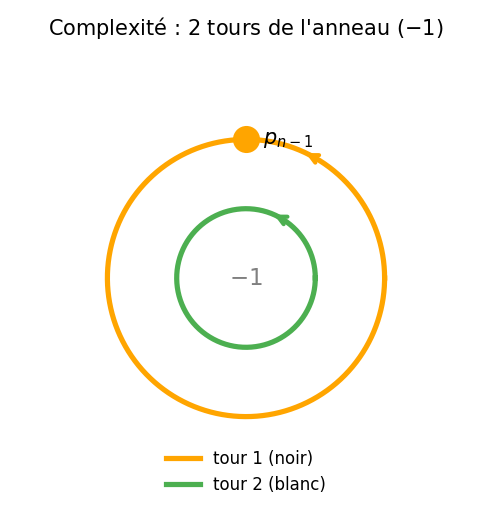
\includegraphics[width=0.42\textwidth]{figures/fig_deux_tours.png}
  \caption{La détection nécessite au plus 2 tours de l'anneau $(-1)$ :
           un premier tour (jeton noir) pour détecter une éventuelle
           contamination, un second tour (jeton blanc) pour confirmer la
           terminaison.}
  \label{fig:deux_tours}
\end{figure}

La latence est donc \textbf{$2(n-1)$ messages de contrôle}.

% ══════════════════════════════════════════════════════
\section{Algorithme de Safia (messages asynchrones)}
% ══════════════════════════════════════════════════════

L'algorithme de Safia étend celui de Dijkstra au cas des
\textbf{transmissions de messages asynchrones}, en utilisant des
\emph{compteurs de message}.

\begin{description}[leftmargin=2.5em]
  \item[$R_1$] Chaque processus maintient un compteur égal à la
               \textbf{différence} entre le nombre de messages de travail
               émis et le nombre de messages de travail reçus.
  \item[$R_2$] Le jeton \textbf{relève les compteurs} lors de sa
               circulation.
\end{description}

\begin{remarque}
  Ces deux règles s'ajoutent aux règles de Dijkstra. Le compteur permet de
  détecter la présence de messages encore en transit dans le canal, même
  lorsque les communications ne sont plus instantanées.
\end{remarque}

\end{document}
